%Research Report in Mechanics
%\documentclass[12pt]{article}
\documentclass[10pt]{article}
\usepackage{latexsym,amsmath}

%\author{blablabla}
%\date{}
%\begin{document}
%\maketitle\documentclass[a4paper,10pt]{article}

\usepackage[utf8x]{inputenc}
%\usepackage[draft]{graphicx}
\usepackage[final]{graphicx}
\usepackage{subfigure}
\usepackage[usenames,dvipsnames]{color}
\usepackage{amsmath}
\usepackage{natbib}
\usepackage{url}
\usepackage{textcomp}
\usepackage[noblocks]{authblk}
%\usepackage{mcode}
% load package with some of the available options - you may not need this!
\usepackage[framed,autolinebreaks]{mcode}
%\usepackage[framed,autolinebreaks]{mcode}

\renewcommand{\vec}[1]{\ensuremath{\boldsymbol #1}}
%\newcommand{\der}[2][]{\ensuremath{\frac{\mathsf{d}{#1}}{\mathsf{d}{#2}}}}
\newcommand{\pder}[2][]{\ensuremath{\frac{\partial{#1}}{\partial{#2}}}}
\newcommand{\scn}[2]{\ensuremath{#1\cdot10^{#2}}}
%\newcommand{\change}[2]{{\color{red}\st{#1}{#2}}}
\newcommand{\change}[2]{{#2}}
\DeclareMathOperator*{\sign}{sign}
\DeclareMathOperator*{\mse}{mse}
\DeclareMathOperator*{\MSE}{MSE}
\DeclareMathOperator*{\RMSE}{RMSE}
\DeclareMathOperator*{\bias}{bias}
\DeclareMathOperator*{\var}{var}
\DeclareMathOperator*{\std}{std}
\DeclareMathOperator*{\cov}{cov}
\DeclareMathOperator*{\mean}{mean}
\DeclareMathOperator*{\median}{median}
\DeclareMathOperator*{\E}{E}
\newcommand{\FT}{\ensuremath{\mathcal F}}
\newcommand{\iFT}{\ensuremath{\mathcal F^{-1}}}
\usepackage{fullpage}
\renewcommand{\lstlistingname}{Example}

\definecolor{mygray}{rgb}{0.35, 0.35, 0.35}
\newcommand{\fa}[0]{\ensuremath{{\color{mygray}I_0}}}
\newcommand{\fb}[0]{\ensuremath{{\color{red}I_1}}}
\newcommand{\fc}[0]{\ensuremath{{\color{blue}I_2}}}
\newcommand{\fd}[0]{\ensuremath{{\color{mygray}I_3}}}

%opening
\title{\vspace*{-1.5cm}
\begin{flushright}
\begin{minipage}{4.5cm}
\tiny{\sc Dept. of Math. \hfill University of Oslo\\Research Report in Mechanics \\ISSN 0801--9940 \hfill May 2016}
\end{minipage}
\end{flushright}
\vskip 1cm Getting started with HydrolabPIV v1.1\thanks{This work was financed by the research project DOMT - Developments in Optical Measurement Technologies (project number 231491 ) funded by the Research Council of Norway.}}
\author[1]{Jostein Kolaas}
\affil[1]{Department of Mathematics, University of Oslo}



\begin{document}
  \maketitle
\section{Short introduction to Particle image velocimetry (PIV)}
There are many ways to measure fluid motion, one of which is particle image velocimetry (PIV).
This is a non-intrusive optical measurement method,
which gives velocity fields resolved in both time and space.
PIV and other similar methods like particle tracking velocimetry (PTV) are based on three principles \citep{Sveen2004}
\begin{enumerate}
 \item A visual representation of fluid motion.
 \item An imaging system for capturing the visual representation.
 \item A method for processing the images to quantify the fluid motion.
\end{enumerate}
To visualize the flow, natural or added tracer particles are usually suspended in the fluid.
While the use of tracer particles is the most common, it is also possible to use dye patterns \citep{Raffel2007}.
If the particles are small and/or neutrally buoyant the particles are deemed passive and will follow the fluid motion.
The imaging system usually consist of a light source, a camera and a lens.
The light source is most commonly a pulsed solid state laser (ND:YAG/ND:YLF), but white light can also be used \citep{Raffel2007}.
Using light sheet optics the laser beams is spread to illuminated the field of view,
which is captured by a high speed digital camera synchronized with the laser, resulting in a sequence of frames 
$\fa$, $\fb$, $\fc$ and $\fd$, see figure \ref{rawseq}.


\begin{figure}[htp]
  \centering
  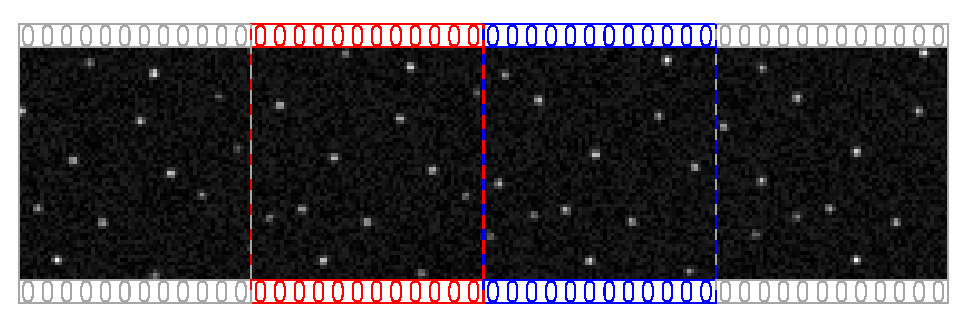
\includegraphics[width=.9\textwidth]{rawsequence20140620}
  \caption{Raw image sequence}
  \label{rawseq}
\end{figure}

Given two images we now want to find an Eulerian description of the velocity field.
We start by dividing images into a regular grid of subwindows, usually with overlap.
%
For each subwindow in the first frame, $\fb$ (see figure \ref{pivptv}a),
we try to match its pattern with a similar pattern in the second frame , $\fc$.
Dividing the optimal match displacement of the pattern by $\Delta t$ we find an ensemble averaged velocity.
%
\begin{figure}[htp]
   \centering  
  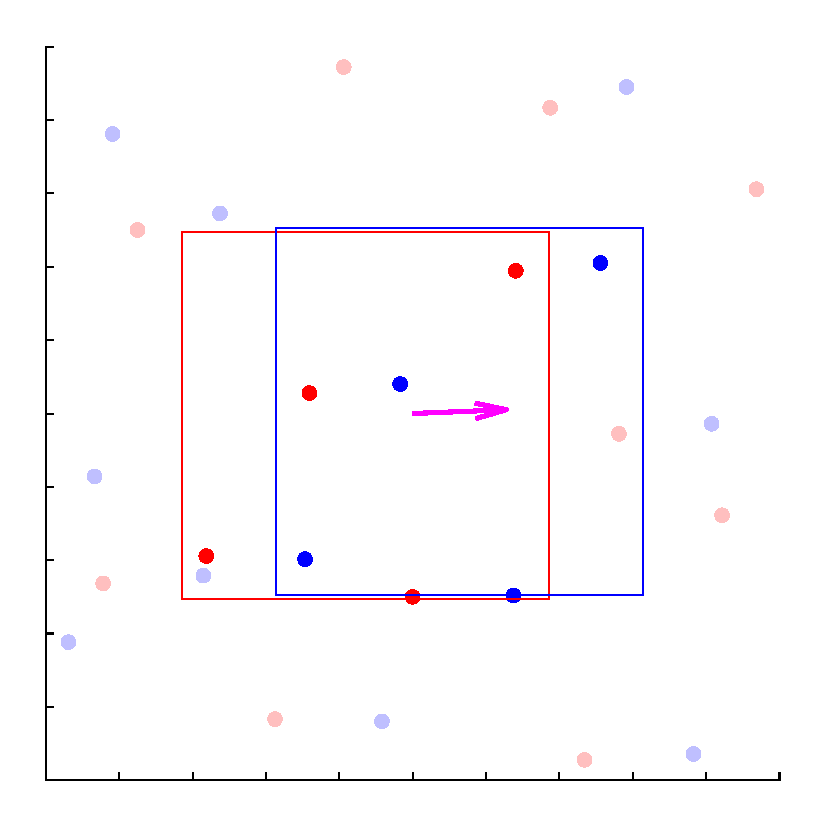
\includegraphics[width=.45\textwidth]{pivoverview20140620}
   \caption{%Principle of particle image velocimetry (PIV) and particle tracking velocimetry (PTV) 
   In PIV the image pattern created by the particles in frame $\fb$ and $\fc$ within the subwindow (rectangles) 
is matched to find an ensemble average {\color{magenta}velocity vector}.}
   \label{pivptv}
\end{figure}
For this we need a metric to tell how different the pattern is, a common choice
is cross-correlation \citep{Willert1991}
\begin{align}
   R_{cc} &= \sum\fb\fc &
   R_{ncc} &= \frac{\sum\fb\fc - \frac{\sum\fb\sum\fc}{N}}
   {\sqrt{\left(\sum\fb^2 - \frac{\left(\sum \fb\right)^2}{N}\right)\left(\sum\fc^2 - \frac{\left(\sum\fc\right)^2}{N}\right) }},
\end{align}
shown with ($R_{ncc}$) and without normalization ($R_{cc}$). 
To speed up processing, fast Fourier transform (FFT) is often used to calculate the cross-correlation.
\cite{Padfield2012} showed that the normalized version also can be done with FFT.
Alternatively, if the image is double exposed, one can auto-correlate the image with itself, see \cite{Adrian1991}.
This enables slower cameras to be used for measurement, but with reduced quality and
there is an ambiguity in the flow direction so it can only be used for unidirectional flow.

To improve the resolution, PIV uses subpixel interpolation to estimate the peak of the difference measure.
This can be done by fitting a quadratic or bi-quadratic polynomial to a 3x3 pixel block around the peak \citep{Nobach2005,Dalziel2012}.
A downside to subpixel interpolation is that it causes peak-locking, an aliasing effect towards whole pixels \citep{Christensen2004}.
It is important to test the experimental setup before measurements to keep this bias error under control.

After the velocity are found, the result can be made more robust by 
checking the quality of the image and difference measure, and 
further validation of the vectors using outlier detection \citep{Westerweel1993,Westerweel2005}.
In more advanced PIV algorithms, multipass methods including distorted passes \citep{Huang1993a,Huang1993b,Scarano2002}, are often used to improve resolution and accuracy.
%\cite{Sveen2004,Raffel2007,Scarano2002}
  \nocite{Kolaas2014}
  
  
  \section{Setup of HydrolabPIV}
  To run HydrolabPIV it needs to be added to the Matlab path:  
  \begin{lstlisting}
addpath(genpath('/mn/kadingir/domt_143903/HydrolabPIV/src'));
addpath('/mn/kadingir/domt_143903/HydrolabPIV/images');
javaaddpath('/mn/kadingir/domt_143903/HydrolabPIV/src/measures');
javaaddpath('/mn/kadingir/domt_143903/HydrolabPIV/src/interp');
  \end{lstlisting}
If necessary replace the folder name with where you installed HydrolabPIV.
%  
If one often uses HydrolabPIV these lines  
can be added to startup.m in the MatLab folder in your home area,
which runs every time MatLab starts.
If this file does not exist you can create it.
  
  \section{Single pass PIV}
  
  
  %\subsection{Simple PIV example}  
  
% \begin{lstlisting}[caption=Hello PIV] 
% im1 = imread('imA.png');
% im2 = imread('imB.png');
%  
% opt = setpivopt(); % Use default options
% piv = normalpass([],im1,[],im2,[],opt);	 
% [U,V,x,y] = replaceoutliers(piv);
%   
% figure;
% scale = 5;
% quiver(x,y,5*U,5*V,0);
%   \end{lstlisting}
%In our first example we will after we have read an image pair,
After we have read an image pair, we will
setup PIV to use 24x24 pixel subwindows with 50\% overlap.
This will give us a velocity vector for every 12 pixels.
The search range should normally be less than half the subwindow size,
in this case we set it to go from -8 to 8 pixels (a third of the subwindow) in both x and y direction.
Other options can also be set using the \emph{setpivopt(\ldots)} function.
The single pass PIV is done with \emph{normalpass(\ldots)} with the  images and options as arguments.
(The empty argument will be explained later).
The result is returned using a structure, which among other things contains the positions (x,y) and the velocities (U,V).
\begin{lstlisting}[caption=Single pass PIV,label=yy] 
im1 = imread('imA.png');
im2 = imread('imB.png');
 
opt = setpivopt('range',[-8 8 -8 8],'subwindow',24,24,.50); 
piv = normalpass([],im1,[],im2,[],opt);
  
figure;
scale = 5;
quiver(piv.x,piv.y,scale*piv.U,scale*piv.V,0);
  \end{lstlisting}
Note that when plotting the vector field it is useful,
especially if comparing vector fields,
to set the scale parameter in \emph{quiver(\ldots)} to zero (avoiding autoscaling).
  
\begin{figure}[htp]
  \centering
  \vspace{0.6cm}
  \subfigure[{\lstlistingname} \ref{yy}]{\includegraphics[width=.4\textwidth]{firstvelocityfield.eps}} \hspace{.1\textwidth}
  \vspace{0.6cm}
  \subfigure[{\lstlistingname} \ref{xx}]{\includegraphics[width=.4\textwidth]{firstvelocityfieldmasked.eps}}
 \caption{Single pass piv with and without masking.}
\end{figure}

In some cases it is useful to mask part of the image,
for instance when the image contains a dynamic free surface. 
The mask is provided as arguments to \emph{normalpass(\ldots)} as another image pair, where 0 is masked and 1 is umasked.
(It is also possible to give a number between 0 and 1 to give less weight to certain pixels).
You can try this out by selecting a few points with \emph{impoly()}, double-click for last point.
\begin{lstlisting}[caption=Single pass PIV with Masking,label=xx] 
% create a polygonal mask 
figure;
imagesc(im1);
set(gca,'Ydir','normal')
h = impoly();
mask = h.createMask();

opt = setpivopt('range',[-8 8 -8 8],'subwindow',24,24,.50); 
piv = normalpass([],im1,mask,im2,mask,opt); 

figure;
scale = 5;
idm = interp2(double(mask),piv.x,piv.y)==1;
quiver(piv.x(idm),piv.y(idm),scale*piv.U(idm),scale*piv.V(idm),0);
\end{lstlisting}

An important step of the PIV measurement process is to check the quality. 
One way is to inspect the signal-to-noise ratio  \emph{piv.snr},
where the noise level is estimated as the median absolute deviation of the correlation/diffrence measure (taken over the whole measure or within the search range)
and the signal strength is the difference between the noise and the peak value.
If the signal-to-noise ratio has a blocky apperance, it would indicate that the particle concentration is to low.
To compansate for this it may be possible to use larger subwindows.
  
Another step in improving the quality of the PIV result is to detect and replace outliers.
For this HydrolabPIV uses 3x3 normalized local median filter \citep{Westerweel2005},
the residuals from the filter is stored in \emph{piv.localres}.
If part of the 3x3 is masked, a masked 5x5 local median filter is used instead.
%
In addition a cubic B-spline is fitted to the velocity field using an iterative weighted least squares fit.
The local residuals are used with the biweight function in the first iteration.
The fit is then iterated a few times where
the residuals normalized by 9x9 local median of the residuals, 
is used to update the weights in the least squares fit.
The normalized residuals form the last iteration are stored in \emph{piv.globalres},
which together with the residuals from the local median filter are used to mark the outliers in \emph{piv.out}.
These outlier can be replaced with \emph{replaceoutliers(\ldots)}, where the missing vectors are evaluated using the fitted B-spline.

\begin{figure}[htp]
  \centering
  \vspace{0.5cm}
  \subfigure[Outlier detection]{\includegraphics[width=.4\textwidth]{firstvelocityfieldoutlier.eps}}
  \\\vspace{0.5cm}
  \subfigure[After replacement of outliers (50\% overlap)]{\includegraphics[width=.4\textwidth]{firstvelocityfieldfixed.eps}}
  \\\vspace{0.5cm}
  %\hspace{.1\textwidth}
  \subfigure[After replacement of outliers (75\% overlap)]{\includegraphics[width=.4\textwidth]{firstvelocityfieldfixed2.eps}}  
 \caption{Outlier detection and replacement ({\lstlistingname} \ref{zz})}
  \label{fig:outlier}
\end{figure}

\begin{lstlisting}[caption=Outlier detection and replacement,label=zz]
im1 = imread('imA.png');
im2 = imread('imB.png');
 
opt = setpivopt('range',[-8 8 -8 8],'subwindow',24,24,.50); 
piv = normalpass([],im1,[],im2,[],opt); 
[U,V,x,y] = replaceoutliers(piv);
  
figure; 
scale = 5; 
quiver(piv.x,piv.y,scale*piv.U,scale*piv.V,0)
hold on; 
idx = not(piv.out);
quiver(piv.x(idx),piv.y(idx),scale*piv.U(idx),scale*piv.V(idx),0)
hold off;
legend(' ok ',' outlier ');
title('Outlier detection');

figure; 
quiver(x,y,scale*U,scale*V,0)
title('Outlier replacement (50% overlap)');

opt2 = setpivopt('range',[-8 8 -8 8],'subwindow',24,24,.75); 
piv2 = normalpass([],im1,[],im2,[],opt2); 
[U2,V2,x2,y2] = replaceoutliers(piv2);

figure;
idx = 1:2:size(U2,2);
quiver(x2(idx,idx),y2(idx,idx),scale*U2(idx,idx),scale*V2(idx,idx),0)
title('Outlier replacement (75% overlap)');
\end{lstlisting}

Note that there are more outliers on the edge, since approximately 50\% of the subwindow is masked.
While for single pass piv vectors on the edge is often ignored, it is important to have
an estimate of velocity on the edge to get high quality displacement when using distorted passes.
%
Since the amount of least squares fit in the B-spline is set to coincide with the subwindow overlap,
a 0\% overlap would result in interpolation of the velocity field and no outlier would be replaced.
Increasing the overlap from 50\% to 75\%  gives 4 times as many vectors resulting in higher computational cost,
but will in general improve the outlier detection and replacement as is shown in figure \ref{fig:outlier}.

\section{Multipass PIV}
  Further improvements in accuracy and resolution can be obtained by using multiple PIV passes, 
  using for instance window shifting or window distortion.
  
  \subsection{Window shifting}
  For a given difference measure the search range is usually maximum half of the subwindow size, limiting the maximum displacement.
  Larger subwindows enables larger maximal displacement/velocity, but at reduced resolution.
  A way to improve the resolution while retaining the maximum displacement is to first use a pass with large subwindows,
  followed by a pass with smaller subwindows shifted by the displacement found in the previous pass as shown in the next example.
          
\begin{lstlisting}[caption=Shallow water wave]
% Read in wave images
im1 = imread('wave1.png');
mask1 = imread('wave1mask.png');
im2 = imread('wave2.png');
mask2 = imread('wave2mask.png');
  
% First pass with masks
opt1 = setpivopt('range',[-8 8 -8 8],'subwindow',64,64,.75);
piv1 = normalpass([],im1,mask1,im2,mask2,opt1); 
[U1,V1] = replaceoutliers(piv1);
 
%Shifted pass using smaller subwindows
opt2 = setpivopt('range',[-4 4 -4 4],'subwindow',32,32,.75);
piv2 = normalpass(piv1,im1,mask1,im2,mask2,opt2);
[U2,V2] = replaceoutliers(piv2);
\end{lstlisting}
\subsection{Window distortion} 
Subwindow based methods like PIV with correlation/difference measure only gives translation,
assuming the velocity field within the subwindow is uniform. To improve accuracy for shear flows,
subwindow distortion \citep{Scarano2002} can be used.
HydrolabPIV finds the distortion of the image pair by
integrating the B-splines fitted to the displacements using Runge-Kutta.
The displacement is then used to interpolate a new image pair tending toward zero/uniform displacement.
Processing this image pair in the regular way gives a correction to the displacements.
%
\begin{lstlisting}[caption=Shallow water wave (continued)]
% Distorted passes
opt3 = setpivopt('range',[-4 4 -4 4],'subwindow',32,32,.75);
piv3 = distortedpass(piv2,im1,mask1,im2,mask2,opt3);
[U3,V3] = replaceoutliers(piv3);
 
opt4 = setpivopt('range',[-4 4 -4 4],'subwindow',32,32,.75);
piv4 = distortedpass(piv3,im1,mask1,im2,mask2,opt4);
[U4,V4,x,y] = replaceoutliers(piv4);                
\end{lstlisting}
% 
To get the best accuracy 3-4 distorted passes are recommended.
%
The default option for estimating distortion uses the standard RK4,
but any other explicit schemes can be used by specifing the Butcher tableau. 
It is also possible to only partially undistort the image pair by setting $\alpha<1$.
\begin{lstlisting}
% partial distort images (half-way) using Heun's method
alpha = 0.5;
opt = setpivopt('tableau',[0 0 0; 1 1 0; 0 1/2 1/2],alpha) 
\end{lstlisting}
An important choice that greatly effects the error is interpolation of the image pair.
\begin{lstlisting}
opt = setpivopt('iminterp',@iminterp2matlab,'linear') % Linear interpolation using matlab
opt = setpivopt('iminterp',@iminterp2matlab,'spline') % Bspline using matlab
opt = setpivopt('iminterp',@iminterp2bsplinej,[])     % Bspline using Java
% Lanczos kernel with 2n-1 lobes using Java
n = 3;
opt = setpivopt('iminterp',@iminterp2lanczosj,n)       
\end{lstlisting}
Lanczos resampling works better for smaller particles $d_p$ = 2-4 pixels while cubic b-spline works better for particls $d_p>$ 5 pixels.
The two Java methods allows for setting the number of computational threads $N$ using \emph{Bspline2(N)} or \emph{Lanczos2(N)}.

 \subsection{Init pass}
If the experiment is time resolved it is possible to save computation time by using previous found velocity fields
as an initial guess to the next image pair using \emph{initpass(\ldots)}.

\begin{lstlisting}[caption=Shallow water wave]
% Read in more wave images
im3 = imread('wave3.png');
mask3 = imread('wave3mask.png');
  
% Use result from previous image pair as initial guess
piv1 = initpass(piv2.Uspline,piv2.Vspline);
 
%Shifted pass using smaller subwindows
opt2 = setpivopt('range',[-4 4 -4 4],'subwindow',32,32,.75);
piv2 = normalpass(piv1,im2,mask2,im3,mask3,opt2);
[U2,V2] = replaceoutliers(piv2);
\end{lstlisting}
  
\section{Coordinate transformations}
To get the physical quanteties we need convert the from the camera coordinate system $x$ in pixel 
to the real world coordinates $\tilde x$.
For this we need a coordinate transformation, the most basic being linear transformation
  \begin{align}
	 \label{eq:lin}
	 \tilde{\vec x} = \begin{bmatrix}\tilde x\\\tilde y\\1\end{bmatrix} &= 
	 \begin{bmatrix} t_{11} & t_{12} & x_0\\ t_{21} & t_{22} & y_0 \\ 0 & 0 & 1\end{bmatrix}
	 \begin{bmatrix}x\\y\\1\end{bmatrix} = T\vec x,
  \end{align}
which include translation, scaling and rotation.
While this transfrom is used for the positions, it becomes necessary to calcuate the Jabobian $J$ to transform the velocity vectors
  \begin{align}
	 \tilde{\vec u} =
	 \begin{bmatrix}\tilde u\\\tilde v\end{bmatrix} &= 
	 \begin{bmatrix}\pder[\tilde x]{x} & \pder[\tilde x]{y}\\ \pder[\tilde y]{x}& \pder[\tilde y]{y} \end{bmatrix}
	 \begin{bmatrix}u\\v\end{bmatrix} = J\vec u \\
\intertext{In the linear case this is rather simple and the Jacobian becomes}
	 J &= \begin{bmatrix} t_{11} & t_{12} \\ t_{21} & t_{22}\end{bmatrix}. 
  \end{align}
%
  Given a set of control points in pixel and world coordinates   
  \begin{align}
	 X' &= \begin{bmatrix}
		x_1 & y_1 & 1\\
	\vdots & \vdots & \vdots \\
	  x_n & y_n & 1 
	 \end{bmatrix} &  
	 {\tilde X}' &= \begin{bmatrix}
		 \tilde x_1 & \tilde y_1 & 1\\
	\vdots & \vdots & \vdots \\
	 \tilde x_n & \tilde y_n & 1
	 \end{bmatrix} 
  \end{align}
  inserting into equation \ref{eq:lin}
  \begin{align}
    \label{eq:lin2}
	 \tilde X &= TX,
  \end{align}
  which can be solved with respect to transformation $T$
  \begin{align}
	 T & = \left[(X')^{-1}({\tilde X}')\right]'.
  \end{align}
  If there are more controlpoints than is needed, we can solve for $T$ in a least squares fashion
  \begin{align}
	 T & = \left[(XX')^{-1}(X{\tilde X}')\right]'.
  \end{align}
 Sometimes a linear transform is not enough to describe the mapping,
 for instance if camera is slight tilted up- or downward we get projective transfrom.
 This can be approximated by Cubic-transformation
     \begin{align}
	 \tilde{\vec x} = \begin{bmatrix}\tilde x\\\tilde y\\1\end{bmatrix} &= 
	 \begin{bmatrix}
		t_{11} & t_{12} & t_{13} & t_{14} & t_{15} & t_{16} & t_{17} & t_{18} & t_{19} & x_0\\ 
		t_{21} & t_{22} & t_{23} & t_{24} & t_{25} & t_{26} & t_{27} & t_{28} & t_{29} & y_0\\
	   0 & 0& 0 & 0 & 0 & 0& 0 & 0 & 0 & 1
	 \end{bmatrix}
	 \begin{bmatrix}x^3\\x^2y\\xy^2\\y^3\\x^2\\xy\\y^2\\x\\y\\1\end{bmatrix} = T\vec x.
  \end{align}
Using the control point matrix
\begin{align}
	 X' &= \begin{bmatrix}
		x_1^3 & x_1^2y_1 & x_1y_1^2 & y_1^3 & x_1^2 & x_1y_1 & y_1^2 & x_1 & y_1 &  1 \\
	\vdots & \vdots & \vdots & \vdots & \vdots & \vdots & \vdots & \vdots & \vdots & \vdots \\
	x_n^3 & x_n^2y_n & x_ny_n^2 & y_n^3 & x_n^2 & x_ny_n & y_n^2 & x_n & y_n &  1 
	 \end{bmatrix},
\end{align}
we can solve for $T$ in a simular fashion as for the linear case. Note that since this transform
is non-linear, ($T$ is not invertible). Also the Jabobian for this transform is slightly more complicated 
as it depends on the position.
  
\begin{figure}[htp]  
  \centering
  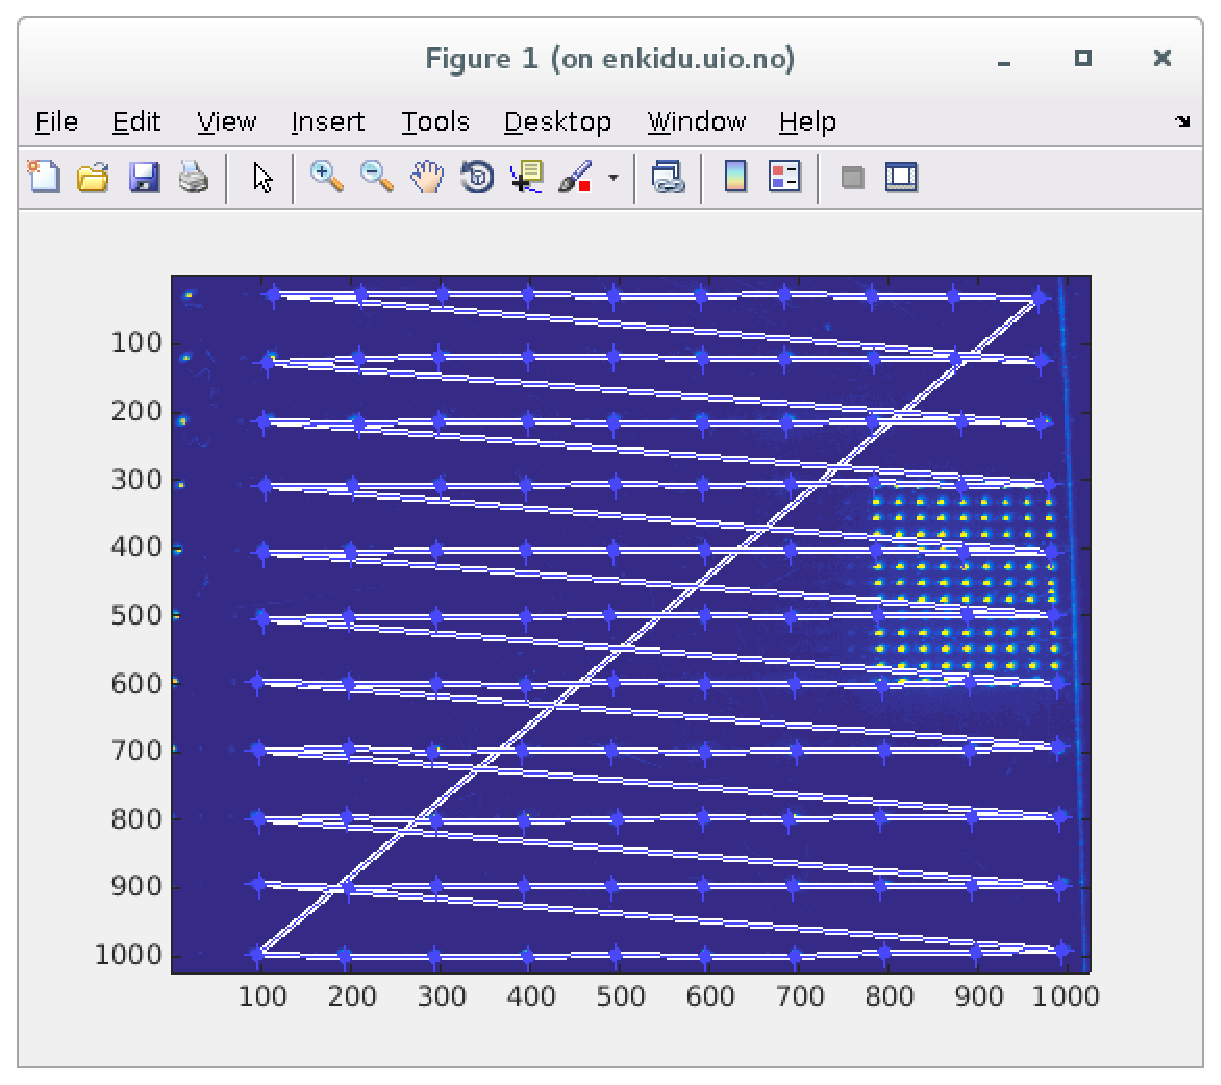
\includegraphics[width=.6\textwidth]{pixelcoord.eps}
  \caption{Selecting pixel reference points ({\lstlistingname} \ref{tform})}
  \label{fig:controlpoints}
\end{figure}
  
 In the Shallow water wave example the camera is slighty tilted upwards to get a better measurement of the surface elevation,
 so we will use a cubic coordinate transformation.
 If we use \emph{ndgrid(\ldots)} to define a grid of world control points, 
 it is convenient to select the pixel control point from right to left, and then upwards, see figure \ref{fig:controlpoints}.
 The last control point is selected with a double-click.
\begin{lstlisting}[caption=Creating a coordinate system,label=tform]
coord = imread('wavecoord.png');
imagesc(coord)
 
% Select reference points in pixel coordinate
h=impoly;
pixel = h.getPosition;

% Refine pixel positions (optional)
c = graythresh(coord);
bw = im2bw(coord);
cc = bwconncomp(bw);
stats = regionprops(cc,'Centroid');
xc = vertcat(stats.Centroid);
idx = knnsearch(xc,pixel);
pixel = xc(idx,:);
 
% Define matching reference points in world coordinate
[wx,wy] = ndgrid((9:-1:0)*0.02 + 4.33,(-10:0)*0.02 + 0.103);
world = [wx(:) wy(:)];
  
% Create coordinate transformation
[tform,err,errinv] = createcoordsystem(pixel,world,'cubic')   
\end{lstlisting}
  
Using this coordinate transformation we can look at the shallow water stokes wave using real world units as seen in figure \ref{fig:waveworld}.
\begin{lstlisting}[caption=Using the coordinate transform,label=wave]
dt = 1/375;
[U4,V4,x,y] = replaceoutliers(piv4,mask1&mask2);     
[Uw,Vw,xw,yw] = pixel2world(tform,U4,V4,x,y,dt);

% Surface 
[idx1,eta1] = max(mask1); 
[idx2,eta2] = max(mask2); 
[etax,etay] = tformfwd(tform,1:1024,(eta1+eta2)/2);

figure;
idx = 1:4:129;
scale = 1/50;
quiver(xw(idx,idx),yw(idx,idx),scale*Uw(idx,idx),scale*Vw(idx,idx),0);
hold on;
plot(etax,etay,'r');
hold off;
xlabel(' x [ m ] ');
ylabel(' y [ m ] ');
\end{lstlisting}

\begin{figure}[htp]  
  \centering
  \includegraphics[width=.6\textwidth]{wave_velocityfield.eps}
  \caption{Top of shallow water Stokes wave from {\lstlistingname} \ref{wave}}
  \label{fig:waveworld}
\end{figure}
  

\section{Ensemble PIV}
In MicroPIV volume illumination is often used, which results in low seeding concentration due to visibility problem \citep{Olsen2000}.
PIV on these type of images has a poor signal-to-noise ratio, and the velocity from PIV becomes noisy, see figure \ref{fig:ensemble}a,c.
To overcome this \cite{Wereley2005} suggest taking an ensemble average of the correlation peaks in time taken over many images,
improving the signal-to-noise ratio and providing an average velocity field, see figure \ref{fig:ensemble}b,d.
%
\begin{figure}[ht]
  \label{fig:ensemble}
  \centering
  \subfigure[Velocity field (single image)]{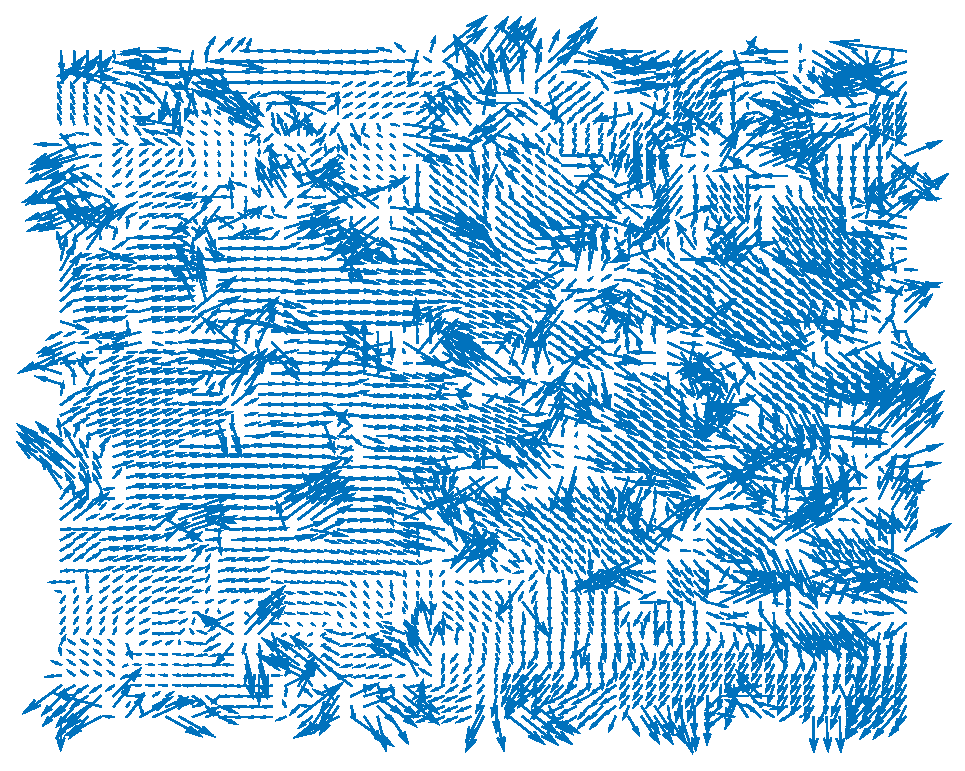
\includegraphics[width=.4\textwidth]{velocityfield_single_image.eps}}\vspace{.2cm} \hspace{.15\textwidth}
  \subfigure[Velocity field (ensemble)]{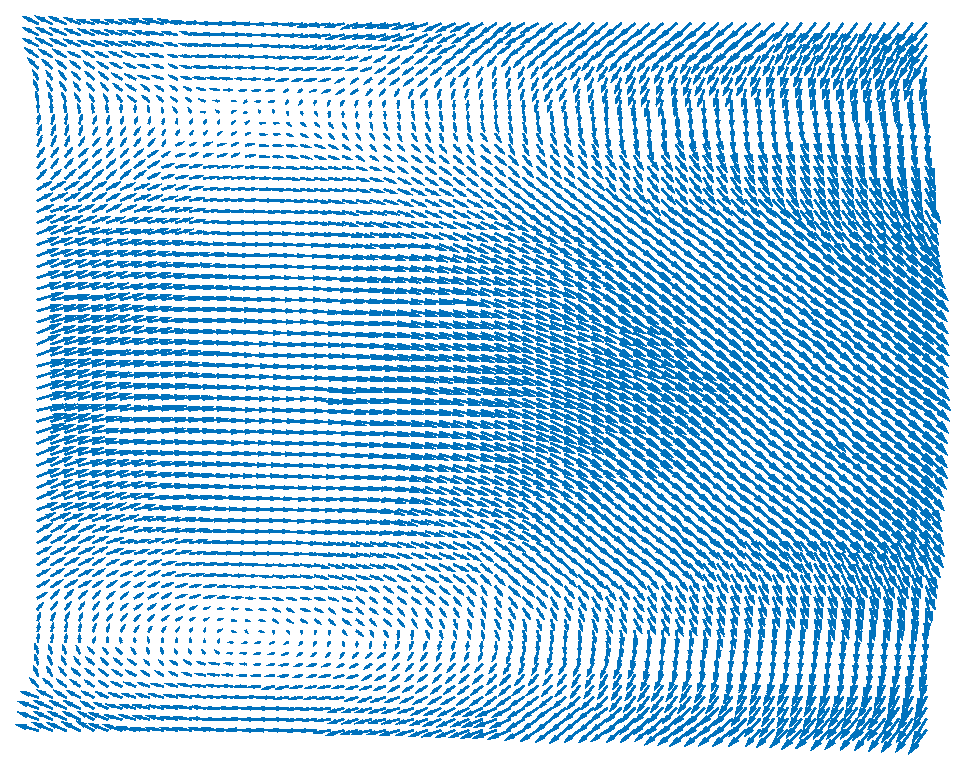
\includegraphics[width=.4\textwidth]{velocityfield_ensemble.eps}} \vspace{.2cm}\\ %\hspace{2cm}
  \subfigure[SNR (single image)]{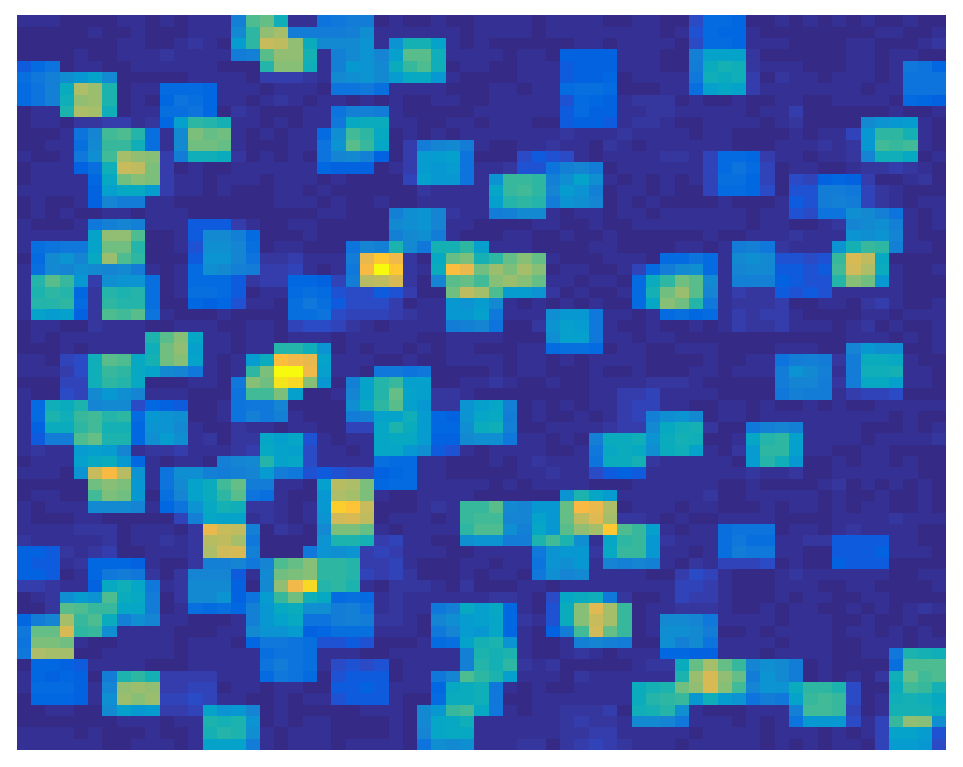
\includegraphics[width=.4\textwidth]{snr_single_image.eps}}\hspace{.15\textwidth} 
  \subfigure[SNR (ensemble)]{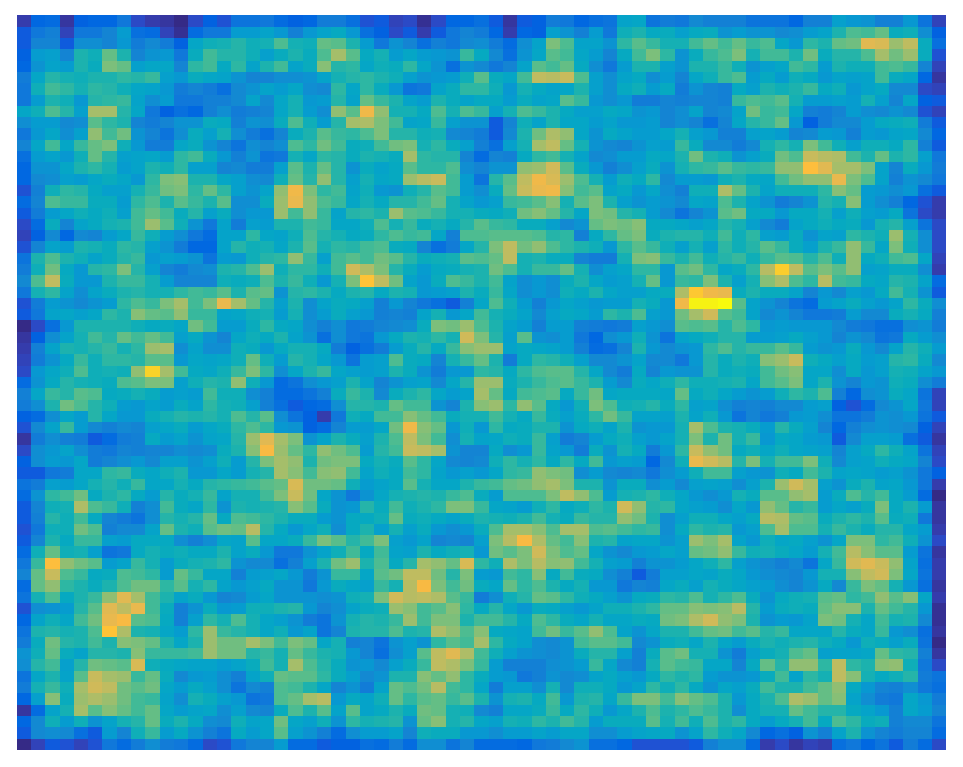
\includegraphics[width=.4\textwidth]{snr_ensemble.eps}}
 \caption{Ensemble PIV}
\end{figure}
%
HydrolabPIV has two ways to perform ensemble PIV. The first way is to provide the images series as a 3D matrix.
\begin{lstlisting}[caption=Ensemble PIV]
% Load images
I=512; J=512; K=25;
im1 = zeros(I,J,K);
im2 = zeros(I,J,K);
for k=1:K
  im1(:,:,k) = imread(sprintf('sparse%02dA.png',k));
  im2(:,:,k) = imread(sprintf('sparse%02dB.png',k));  
end

opt = setpivopt('ensemble',@nanmedian);
piv = normalpass([],im1,[],im2,[],opt);
[U,V,x,y] = replaceoutliers(piv);

figure;
quiver(x,y,U,V);
\end{lstlisting}
This has the advantage that it can be made more robust by setting median as the ensemble function.
Also note that color images will be seen as an ensemble average over the color channels.
%
The second way is to read in the image pairs sequentially with multiple calls to normalspass.
This requires less memory, but is limited to using mean as ensemble function.
\begin{lstlisting}[caption=Ensemble PIV (alternative)]
opt1 = setpivopt('savepeaks',true);
for k=1:25
  im1 = imread(sprintf('sparse%02dA.png',k));
  im2 = imread(sprintf('sparse%02dB.png',k));
  
  if(k==1)    
    piv1 = normalpass([],im1,[],im2,[],opt1);
  else
    piv1 = normalpass([],im1,[],im2,[],piv1);
  end
end
[U1,V1,x1,y1] = replaceoutliers(piv1);

figure;
quiver(x1,y1,U1,V1);
\end{lstlisting}
To make a compromise between memory and robustness, both of the methods can be combined.
Increasing the accuracy is also possible using multipass ensemble PIV, including distorted passes.
\begin{lstlisting}[caption=Multipass ensemble PIV]
opt2 = setpivopt('savepeaks',true,'savedisplacements',true);
for k=1:25
  im1 = imread(sprintf('sparse%02dA.png',k));
  im2 = imread(sprintf('sparse%02dB.png',k));
  
  if(k==1)    
    piv2 = distortedpass(piv1,im1,[],im2,[],opt2);
  else
    piv2 = distortedpass(piv1,im1,[],im2,[],piv2);
  end
end
[U2,V2,x2,y2] = replaceoutliers(piv2);
\end{lstlisting}
    
%   \section{Preprocessing}
% 	 \begin{itemize}
% 	  \item Min-max filter
% 	 \end{itemize}
%   \section{Postprocessing}
% 	 \begin{itemize}
% 	  \item vorticity
% 	  \item vortex detection
% 	 \end{itemize}
% 
\section{Measure functions}
 To match the pattern in a subwindow pair a measure function is needed, in PIV this is
 most often cross-correlation, but other options like minimum quadratic difference are also available.
 The measure function can be set in HydrolabPIV using
\begin{lstlisting}
opt = setpivopt(..., 'measure', @mfun, mparam, @prefun, ...)  
\end{lstlisting}
  where $mfun$ can be one of several measures included with HydrolabPIV or a custom function:
\begin{lstlisting}
[dm,mm] = mfun(f1,m1,f2,m2,idh,idw,mparam)   
\end{lstlisting}   
  Given two subwindows with masks $f_1$/$m_1$ and $f_2$/$m_2$ with sizes ($i$,$j$) and $(k,l)$
  respectively, $@mfun$ should return a measure, dm, with zero 
  displacement peak located in the center and  the masked fraction, mm,
  both of size $(i+k-1)\times(j+l-1)$. The indices $(idh,idw)$ show which part of 
  the difference measure is needed. 
  $mparam$ provides an additional argument to the $@mfun$ function, see
  specific $mfun$ function for it usage. 
  The function $@prefun$ is applied to the measure before subpixel interpolation. 
  For cross-correlation this can be for instance $@log$, practically assuming the measure peak is   
  Gaussian when using quadratic fit in subpixel interpolation  
 \subsection{Cross-correlation}
 The most common measure used in PIV is cross-correlation.
   \begin{align*}	 
	 cc(r,s) &= \frac{1}{IJ}\sum_{i,j} {f_1}_{(i+r,j+s)}\cdot {f_2}_{(i,j)},
  \end{align*}
  often calculated with fast Fourier transform  
  \begin{align*}	 
	 cc = \frac{1}{IJ}\iFT\left(\FT(f_1)\cdot\FT(f_2^*)\right).
  \end{align*}    
  To improves the bias error for partially masked subwindows (including the edges of the image),
  HydrolabPIV uses masked/weighted cross-correlation  
  \begin{align*} 
	 mcc(r,s) &= \frac{\sum_{i,j} \left({m_1}_{(i+r,j+s)}\cdot {f_1}_{(i+r,j+s)}\right)
	                         \cdot\left({m_2}_{(i,j)}\cdot {f_2}_{(i,j)}\right)}
	                         {\sum_{i,j} {m_1}_{(i+r,j+s)}\cdot {m_2}_{(i,j)}},
  \end{align*}
  which also can be calculate with fast Fourier transform 
  \begin{align*} 
	 mcc &= \frac{\iFT\left(\FT(m_1\cdot f_1)\cdot\FT(m_2^*\cdot f_2^*)\right)}{\iFT\left(\FT(m_1)\cdot\FT(m_2^*)\right)}.
  \end{align*}  
To achieve higher accuracy it is possible to use normalized cross-correlation
\begin{align*}
  ncc(r,s) &= \frac{num(r,s)}{\sqrt{den_1(r,s)\cdot den_2}}, \\
\intertext{where}
	 num(r,s) &= \sum_{i,j} {f_1}_{(i+r,j+s)}\cdot {f_2}_{(i,j)}  - \frac{\sum_{i,j} {f_1}_{(i+r,j+s)}\sum_{i,j}{f_2}_{(i,j)}}{IJ}, \\
	 den_1(r,s) &= \sum_{i,j} {f_1}_{(i+r,j+s)}^2  - \frac{\left(\sum_{i,j} {f_1}_{(i+r,j+s)}\right)^2}{IJ}, \\
	 den_2 &= \sum_{i,j} {f_2}_{(i,j)}^2  - \frac{\left(\sum_{i,j} {f_2}_{(i,j)}\right)^2}{IJ}.
\end{align*}
Note that $den_2$ is constant and is sometimes left out of the calculation as it is only a scaling factor.
In a similar way the normalized cross-correlation can be
generalized to a masked/weighted normalized cross-correlation 
\begin{align*}
  mncc(r,s) &= \frac{num(r,s)}{\sqrt{den_1(r,s)\cdot den_2(r,s)}} \\
\intertext{where}
	 num(r,s) &= \sum_{i,j} \left({m_1}_{(i+r,j+s)}\cdot {f_1}_{(i+r,j+s)}\right)\cdot\left( {m_2}_{(i,j)}\cdot {f_2}_{(i,j)}\right) \\
	 &-\frac{\sum_{i,j} {m_2}_{(i,j)}\cdot\left({m_1}_{(i+r,j+s)}\cdot {f_1}_{(i+r,j+s)}\right)\sum_{i,j} {m_1}_{(i+r,j+s)}\cdot \left({m_2}_{(i,j)}\cdot {f_2}_{(i,j)}\right)}
	 {\sum_{i,j} {m_1}_{(i+r,j+s)}\cdot {m_2}_{(i,j)}} \\
	 den_1(r,s) &= \sum_{i,j} {m_2}_{(i,j)}\cdot\left({m_1}_{(i+r,j+s)}\cdot {f_1}_{(i+r,j+s)}^2\right)  
	 -\frac{\left(\sum_{i,j} {m_2}_{(i,j)}\cdot\left({m_1}_{(i+r,j+s)}\cdot {f_1}_{(i+r,j+s)}\right)\right)^2}{\sum_{i,j} {m_1}_{(i+r,j+s)}\cdot {m_2}_{(i,j)}} \\
	 den_2(r,s) &= \sum_{i,j} {m_1}_{(i+r,j+s)}\cdot\left({m_2}_{(i,j)}\cdot {f_2}_{(i,j)}^2\right)
	 -\frac{\left(\sum_{i,j} {m_1}_{(i+r,j+s)}\cdot\left({m_2}_{(i,j)}\cdot {f_2}_{(i,j)}\right)\right)^2}{\sum_{i,j} {m_1}_{(i+r,j+s)}\cdot {m_2}_{(i,j)}} 
\end{align*}
Note that when a mask is present $den_2$ is not constant with respect to $r$,$s$ anymore and should be included.
Using this form also enables calculating the masked/weighted normalized cross-correlation with fast Fourier transform \citep{Padfield2012}
\begin{align*}
  mncc &= \frac{num}{\sqrt{den_1\cdot den_2}}, \\
\intertext{where}
	 num &= \iFT(F_1\cdot F_2) - \frac{\iFT(M_1\cdot F_2)\iFT(M_2\cdot F_1)}{\iFT(M_1\cdot M_2)}, \\
	 den_1 &= \iFT(M_2\cdot\FT(m_1\cdot (f_1)^2))   - \frac{\left(\iFT(M_2\cdot F_1)\right)^2}{\iFT(M_1\cdot M_2)}, \\
	 den_2 &= \iFT(M_1\cdot\FT(m_2\cdot (f_2^*)^2)) - \frac{\left(\iFT(M_1\cdot F_2)\right)^2}{\iFT(M_1\cdot M_2)},
  \end{align*}
$F_1=\FT(m_1\cdot f_1)$, $M_1=\FT(m_1)$, $F_2=\FT(m_2^*\cdot f_2^*)$ and $M_2=\FT(m_2^*)$.
When all the masks values are one, this can be used to calculate the regular normalized cross-correlation as well.
%
The fast Fourier transform based cross-corrections methods can be used by setting
\begin{lstlisting}
  opt = setpivopt('measure',@regularcc,true,@log);   
  opt = setpivopt('measure',@maskedcc,true,@log);   
  opt = setpivopt('measure',@maskedncc,true,@(x) x);  
\end{lstlisting}
The subwindows are padded before FFT evaluation, but can be turn off by using mparam (increased speed, less accuracy).
It is possible to apply the log function to the difference measure before the subpixel 
interpolation, but this is not recommended for normalized cross-correlation,
see subsection \ref{subpixel} for more information.
Under some condition, calculation direct sums is faster, which can be done by setting
\begin{lstlisting}
  opt = setpivopt('measure',@maskednccj,[],@(x) x);
  opt = setpivopt('measure',@maskedccj,[],@(x) x);
\end{lstlisting}
Mparam is not used in these cases.
  
% \subsection{Phase-correlation}
% 
% 
%   \begin{align*}	 
% 	 pc = \iFT\left(\frac{\FT(f_1)\cdot\FT(f_2^*)}{\left|\FT(f_1)\cdot\FT(f_2^*)\right|^\alpha}\right)
%   \end{align*}
%   
%   \begin{lstlisting}
%    opt = setpivopt('measure',@phasecorr,alpha,@(x) x);    
%    \end{lstlisting}
\subsection{Minkowski differences}
Other measures have been used for PIV, for instance \cite{Gui1998} used  Minimum quadratic difference, which is a special case of the Minkowski differences 
   \begin{align*}
		md_{(r,s;\alpha)} = \left\lgroup\frac{1}{IJ}\sum_{i,j} \left|{f_1}_{(i+r,j+s)}-{f_2}_{(i,j)}\right|^\alpha\right\rgroup^{1/\alpha}.
   \end{align*} 
These also exist in a masked/weighted version
\begin{align*}
		mmd_{(r,s;\alpha)} = \left[\frac{\sum_{i,j} w\left|{f_1}_{(i+r,j+s)}-{f_2}_{(i,j)}\right|^\alpha}
		{ \sum_{i,j} w}\right]^{1/\alpha},
\end{align*}
where  $w = {m_1}_{(i+r,j+s)}\cdot {m_2}_{(i,j)}$, 
and a normalized version 
\begin{align*}
		mnmd_{(r,s;\alpha)} = \left[\frac{\sum_{i,j} w\left|{f_1}_{(i+r,j+s)}-{f_2}_{(i,j)}\right|^\alpha}
		{ \sqrt{\left(\sum_{i,j} w\left|{f_1}_{(i+r,j+s)}\right|^\alpha\right)\cdot\left(\sum_{i,j} w\left|{f_2}_{(i,j)}\right|^\alpha\right)}}\right]^{1/\alpha},
\end{align*}
introduced in DigiFlow by \cite{Dalziel2012}. 
%
The masked/weighted or normalized Minkowski differences can be used by setting:
\begin{lstlisting}
  opt = setpivopt('measure',@maskedmdj,alpha,@(x) -x);
  opt = setpivopt('measure',@maskednmdj,alpha,@(x) -x);
\end{lstlisting}
With the exception of some of the special cases this is a rather slow measure due to the usage of power function.
Note the use of $-x$ to find the minimum value rather than a maximum peak value as for cross-correlation.


% \begin{align*}
% 		mnmd = \sqrt{\frac{\sum_{i,j}w\cdot f_1^2 - 2w\cdot f_1\cdot f_2 +w\cdot f_2^2}
% 		{ \sqrt{\left(\sum_{i,j} w\cdot f_1^2\right)\cdot\left(\sum_{i,j} w\cdot f_2^2\right)}}}
% \end{align*}

\subsubsection{Geometric difference ($\alpha\rightarrow 0$)}
The first special case is when $\alpha\rightarrow 0$ 
\begin{align*}
 md_{(r,s;\alpha\rightarrow 0)} = \left[\prod_{i,j} \left|{f_1}_{(i+r,j+s)}-{f_2}_{(i,j)}\right|\right]^{1/IJ}
\end{align*}
and is mostly provided for academic interest.
Nevertheless it gives some insight into what happens for smaller values of $\alpha$.
Due to the product nature of the measure, it is sensitive to broadbanded noise in the image.
It is recommended convert integer images to floating point and add small amount of noise, 
since the measure fails if ${f_1}_{(i+r,j+s)}={f_2}_{(i,j)}$ for any $i$ and $j$.
The masked/weighted of the geometric difference measure is
\begin{align*}
 mmd_{(r,s;\alpha\rightarrow 0)} = \left[\prod_{i,j} \left|{f_1}_{(i+r,j+s)}-{f_2}_{(i,j)}\right|^w\right]^{1/\sum_{i,j} w}
\end{align*}
and its normalized version
\begin{align*}
 mnmd_{(r,s;\alpha\rightarrow 0)} = \left[\frac{\prod_{i,j} \left|{f_1}_{(i+r,j+s)}-{f_2}_{(i,j)}\right|^w}
 {\sqrt{\left(\prod_{i,j} \left|{f_1}_{(i+r,j+s)}\right|^w\right)
   \cdot\left(\prod_{i,j} \left|{f_2}_{(i,j)}\right|^w\right)}}\right]^{1/\sum_{i,j} w}.
\end{align*}
The Normalized also fails if ${f_1}_{(i+r,j+s)}=0$ or ${f_2}_{(i,j)}=0$ for any $i$ and $j$,
but this is easily fixed by adding some noise or a small constant.
Note that the geometric difference measure can also be evaluated as a sum rather than a product using the log function.

\subsubsection{Minimum absolute difference ($\alpha=1$)}
Minimum absolute difference used for PIV by \cite{Gui1997} 
and is the only Minkowkski difference measure with some claim to robustness, 
which might be useful when out-of-plane loss of particles is present.
   \begin{align*}
		md_{(r,s;\alpha=1)} = \frac{1}{IJ}\sum_{i,j} \left|{f_1}_{(i+r,j+s)}-{f_2}_{(i,j)}\right|
   \end{align*}  
It also has the least number of operation in its direct form, but practically the speed difference is neglectable.
The masked/weighted version is
\begin{align*}
		mmd_{(r,s;\alpha=1)} = \frac{\sum_{i,j} w\left|{f_1}_{(i+r,j+s)}-{f_2}_{(i,j)}\right|}{\sum_{i,j} w},
\end{align*}
and its normalized form is
\begin{align*}
		mnmd_{(r,s;\alpha=1)} = \frac{\sum_{i,j} w\left|{f_1}_{(i+r,j+s)}-{f_2}_{(i,j)}\right|}
		{ \sqrt{\left(\sum_{i,j} w\left|{f_1}_{(i+r,j+s)}\right|\right)\cdot\left(\sum_{i,j} w\left|{f_2}_{(i,j)}\right|\right)}}.
\end{align*}
\subsubsection{Minimum quadratic difference ($\alpha=2$)}
Minimum quadratic difference 
   \begin{align*}
		md_{(r,s;\alpha=2)} = \sqrt{\frac{1}{IJ}\sum_{i,j} \left({f_1}_{(i+r,j+s)}-{f_2}_{(i,j)}\right)^2}
   \end{align*}
was used with PIV by \cite{Gui1998}.
Its masked/weighted version is
\begin{align*}
		mmd_{(r,s;\alpha=2)} = \sqrt{\frac{\sum_{i,j} w\left({f_1}_{(i+r,j+s)}-{f_2}_{(i,j)}\right)^2}
		{ \sum_{i,j} w}}.
\end{align*}
This can be rewritten as
\begin{align*}
		mmd_{(r,s;\alpha=2)} = \sqrt{\frac{\sum_{i,j} w\cdot {f_1}_{(i+r,j+s)}^2 -2w\cdot{f_1}_{(i+r,j+s)}\cdot{f_2}_{(i,j)}  + w\cdot{f_2}_{(i,j)}^2 }
		{ \sum_{i,j} w}}
\end{align*}
which can be implemented with FFT using the same methods as for normalized cross-corrections,
\begin{align*}
	 mmd_{(\alpha=2)} = \sqrt{\frac{\iFT(\FT(m_1\cdot(f_1)^2)\cdot M_2) - 2\iFT(F_1\cdot F_2) + \iFT(M_1\cdot\FT(m_2^*\cdot(f^*_2)^2))}
	 {\iFT\left(M_1\cdot M_2\right)}}
\end{align*}  
$F_1=\FT(m_1\cdot f_1)$, $M_1=\FT(m_1)$, $F_2=\FT(m_2^*\cdot f_2^*)$ and $M_2=\FT(m_2^*)$.
Note that the middle term is essentially is the cross-correlation. The Normalized minimum quadratic difference is
\begin{align*}
		mnmd_{(r,s;\alpha=2)} = \sqrt{\frac{\sum_{i,j} w\left({f_1}_{(i+r,j+s)}-{f_2}_{(i,j)}\right)^2}
		{ \sqrt{\left(\sum_{i,j} w\cdot{f_1}_{(i+r,j+s)}^2\right)\cdot\left(\sum_{i,j} w\cdot{f_2}_{(i,j)}^2\right)}}},
\end{align*}
which can also implemented using FFT
\begin{align*}
	 mnmd_{(\alpha=2)} = \sqrt{\frac{\iFT(\FT(m_1\cdot(f_1)^2)\cdot M_2) - 2\iFT(F_1\cdot F_2) + \iFT(M_1\cdot\FT(m_2^*\cdot(f^*_2)^2))}
	 {\sqrt{\iFT(\FT(m_1\cdot(f_1)^2)\cdot M_2) \cdot \iFT(M_1\cdot\FT(m_2^*\cdot(f^*_2)^2))}}}
\end{align*}
Note that it does not require any more FFTs for the normalization, requiring fewer FFTs than normalized cross-corrections, 
making it the fastest of the normalized measures. The FFT based versions can be used in HydrolabPIV by setting:
\begin{lstlisting}
opt = setpivopt('measure',@maskedmqd,true,@(x) -x);
opt = setpivopt('measure',@maskednmqd,true,@(x) -x);   
\end{lstlisting}
\subsubsection{Minimum maximum difference ($\alpha\rightarrow\infty$)}
The last special case is the minimum maximum difference
\begin{align*}
	md_{(r,s;\alpha\rightarrow\infty)} = \max_{i,j} \left|{f_1}_{(i+r,j+s)}-{f_2}_{(i,j)}\right|,
\end{align*}
which  works well with noisy images, but is sensitive to outliers in the image, 
for instance hotpixels or loss of particles due to both in-plane and out-of-plane motion.    
%   \begin{align*}
% 		mmd_{(r,s;\alpha\rightarrow\infty)} = \max_{i,j} \lceil w\rceil\left|{f_1}_{(i+r,j+s)}-{f_2}_{(i,j)}\right|
%    \end{align*}
As allways it exists in a masked/weighted 
\begin{align*}
	mmd_{(r,s;\alpha\rightarrow\infty)} = \max_{i,j} \left(\sign(w)\left|{f_1}_{(i+r,j+s)}-{f_2}_{(i,j)}\right|\right),
\end{align*}
and normalized form
%    \begin{align*}
% 		mnmd_{(r,s;\alpha\rightarrow\infty)} = \frac{\max_{i,j} \lceil w\rceil\left|{f_1}_{(i+r,j+s)}-{f_2}_{(i,j)}\right|}
% 		{\sqrt{\left(\max_{i,j} \lceil w\rceil\left|{f_1}_{(i+r,j+s)}\right|\right)
% 		\cdot \left(\max_{i,j} \lceil w\rceil\left|{f_2}_{(i,j)}\right|\right)}}
%    \end{align*}

 \begin{align*}
		mnmd_{(r,s;\alpha\rightarrow\infty)} = \frac{\max_{i,j} \left(\sign(w)\left|{f_1}_{(i+r,j+s)}-{f_2}_{(i,j)}\right|\right)}
		{\sqrt{\left(\max_{i,j}\left(\sign(w)\left|{f_1}_{(i+r,j+s)}\right|\right)\right)
		\cdot \left(\max_{i,j} \left(\sign(w)\left|{f_2}_{(i,j)}\right|\right)\right)}}.
   \end{align*}
   
  
   

\begin{figure}[htp]
  \centering  
  \centering
  %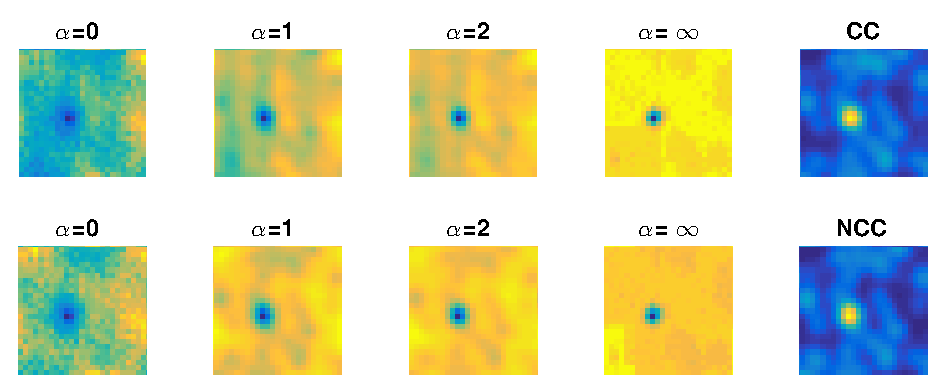
\includegraphics[width=1.00\textwidth]{diffmeasures_peaks2.eps}
  \subfigure[Measures]{\begin{tabular}{ccccc}
    $\alpha\rightarrow0$ & $\alpha=1$ & $\alpha=2$ & $\alpha\rightarrow\infty$ & CC \\
    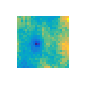
\includegraphics[width=.15\textwidth]{measureimages/F1.eps} &
    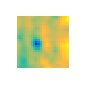
\includegraphics[width=.15\textwidth]{measureimages/F2.eps} &
    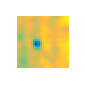
\includegraphics[width=.15\textwidth]{measureimages/F3.eps} &
    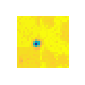
\includegraphics[width=.15\textwidth]{measureimages/F4.eps} &
    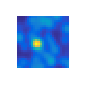
\includegraphics[width=.15\textwidth]{measureimages/F5.eps} \\
    $\alpha\rightarrow0$ & $\alpha=1$ & $\alpha=2$ & $\alpha\rightarrow\infty$ & NCC \\
    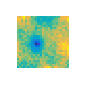
\includegraphics[width=.15\textwidth]{measureimages/F1n.eps} &
    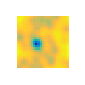
\includegraphics[width=.15\textwidth]{measureimages/F2n.eps} &
    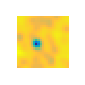
\includegraphics[width=.15\textwidth]{measureimages/F3n.eps} &
    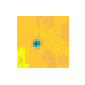
\includegraphics[width=.15\textwidth]{measureimages/F4n.eps} &
    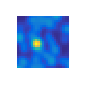
\includegraphics[width=.15\textwidth]{measureimages/F5n.eps} \\
  \end{tabular}}
  \subfigure[U component of velocity, single pass with no outlier replacements]{\begin{tabular}{ccccc}
    $\alpha\rightarrow0$ & $\alpha=1$ & $\alpha=2$ & $\alpha\rightarrow\infty$ & CC \\
    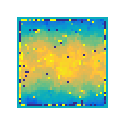
\includegraphics[width=.15\textwidth]{measureimages/U1.eps} &
    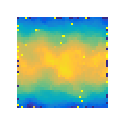
\includegraphics[width=.15\textwidth]{measureimages/U2.eps} &
    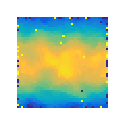
\includegraphics[width=.15\textwidth]{measureimages/U3.eps} &
    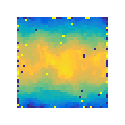
\includegraphics[width=.15\textwidth]{measureimages/U4.eps} &
    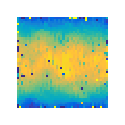
\includegraphics[width=.15\textwidth]{measureimages/U5.eps} \\
    $\alpha\rightarrow0$ & $\alpha=1$ & $\alpha=2$ & $\alpha\rightarrow\infty$ & NCC \\
    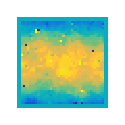
\includegraphics[width=.15\textwidth]{measureimages/U1n.eps} &
    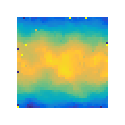
\includegraphics[width=.15\textwidth]{measureimages/U2n.eps} &
    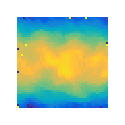
\includegraphics[width=.15\textwidth]{measureimages/U3n.eps} &
    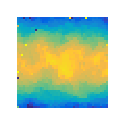
\includegraphics[width=.15\textwidth]{measureimages/U4n.eps} &
    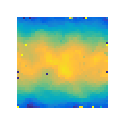
\includegraphics[width=.15\textwidth]{measureimages/U5n.eps} \\
  \end{tabular}}
  %\subfigure[Measures]{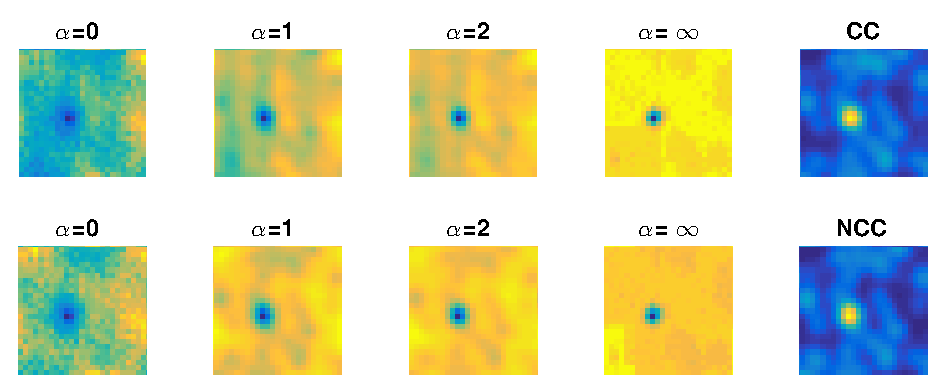
\includegraphics[width=\textwidth]{diffmeasures_peaks2.eps}}\\\vspace{.5cm}
  %\subfigure[U component of velocity, single pass with no outlier replacements]{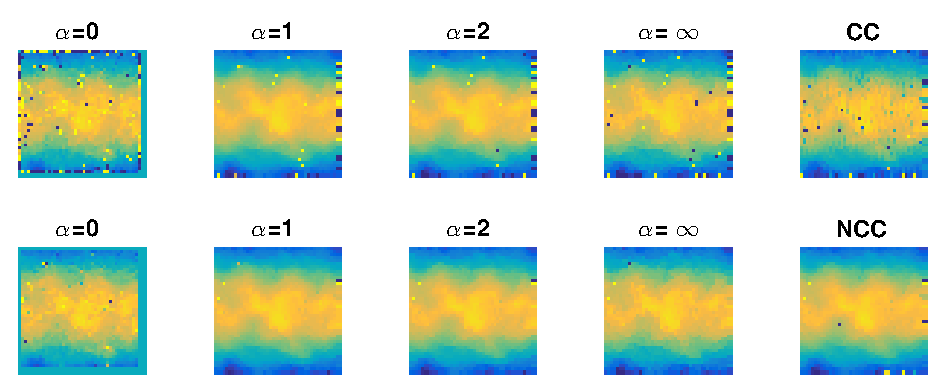
\includegraphics[width=\textwidth]{diffmeasures_velocity2.eps}}
  \caption{Minkowkski difference measures and cross-correlation. Normalized version below.}
\end{figure}

   
\subsection{Subpixel interpolation}
\label{subpixel}
To gain increased accuracy PIV uses subpixel interpolation, based on assumptions of how small particles are
imaged. The first PIV codes used two 1D quadratic fit using 3 points \cite{Raffel2007}, one in each velocity component.
These subpixel interpolation are based on Newtons method with one iteration for finding the peak. 
To increase the accuracy of the peak position further, one can apply a preconditioner to accelerate the convergence,
for instance if the peak is assumed to be Gaussian, the Newton method should converge in one iteration
if the $log$ functions is applied to the measures before subpixel interpolation \citep{Willert1991}.
Note that when peak is iteratively found using multipass with distorted passes, the use of $log$ is not that important.
While 1D subpixel does work, the idea should be generalized to 2D 
using a 3x3 bi-quadratic fit or 3x3 quadratic least squares fit to reduce bias errors \citep{Nobach2005}.
As an alternative to using the $log$ function, a nonlinear least squares fit to a Gaussian using Levenberg-Marquardt is also provided.
There is also 5x5 version of the quadratic least squares and nonlinear least squares fit, these 
often give less outliers but with little or no increase in accuracy.
Outliers caused by the subpixel interpolation are usually due to the Newton iteration diverging 
and are easily detected and replaced by the outlier filter.
The subpixel interpolation in HydrolabPIV is set using:
\begin{lstlisting}
 opt = setpivopt(..., 'subpixel', @subpixelfun, ...) 
\end{lstlisting}
for example using these functions
  \begin{lstlisting}
opt = setpivopt('subpixel',@subpixel3x2)
opt = setpivopt('subpixel',@subpixel3x3)
opt = setpivopt('subpixel',@subpixel3x3ls)
opt = setpivopt('subpixel',@subpixel3x3lm)
opt = setpivopt('subpixel',@subpixel5x5ls)
opt = setpivopt('subpixel',@subpixel5x5lm)
opt = setpivopt('subpixel',@subpixelnone)
\end{lstlisting}
As with the measure function, the subpixel interpolation can be set using a custom function  
\begin{lstlisting} 
  [x0,delta,out] = subpixelfun(F)
\end{lstlisting}
where the $subpixelfun$ should return the integer position from the top corner, $x0$, 
the subpixel correction, $delta$, and an indication whether the method 
believes the result is valid ($out=1$) or an outlier ($out=0$). 

  


   
   
   
   

  %\appendix
  %\section{FAQ}
  %\section{Function reference}
  
  
    
  \bibliography{hlpiv}
\bibliographystyle{spbasic}
\end{document}

